\label{chapter:ModelExecution}
The steps in our model excution  workflow are:
\begin{enumerate}
    \item Run \mfus to create the new project output files (e.g.\ time-varying hydraulic head, drawdown etc).\label{step:modflow}
    \item Run \mut\ to post-process the Modflow project, which produces \tecplot\ output files for the various Modflow domains (i.e.\ \gwf, \swf\ and/or \cln ) created during the Modflow simulation.\label{step:mut2}
    \item Run \tecplot\ and examine the Modflow output files.   \label{step:Tecplot2}
\end{enumerate}

To run \mfus\ on the \texttt{1\_VSF\_Column} example, and assuming we have a command prompt open at the appropriate directory, we can type:
\begin{verbatim}
    usgs_1 modflow
\end{verbatim}
which obtains the prefix for the \mfus\ input files, in this case the default prefix {\sf modflow}.

 As \mfus\ processes the input file, output is written to the screen:

        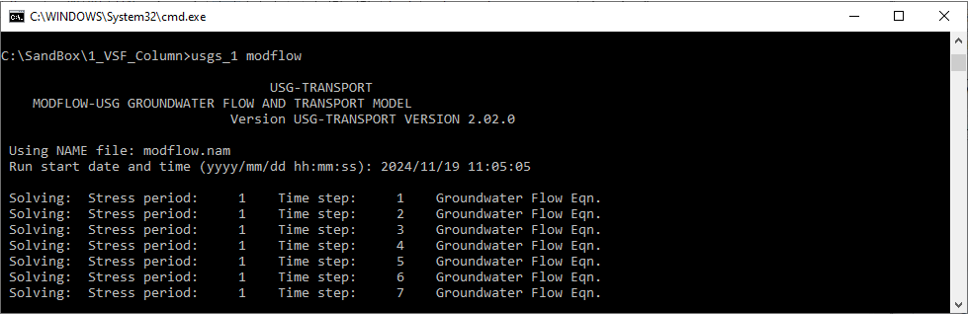
\includegraphics[width=\textwidth]{4_1_RunScreen}

 If execution is successful you will see the {\sf Normal termination of simulation} message:

        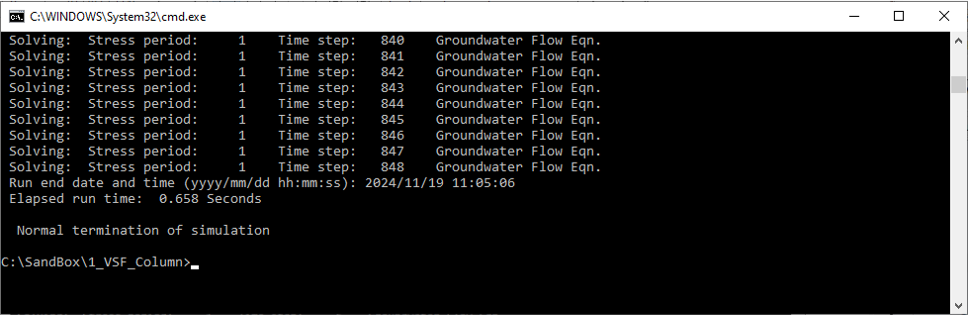
\includegraphics[width=\textwidth]{4_1_RunScreenExit}

 Every \mfus\ simulation generates a run-time
listing file, in this case called {\tt modflow.lst}, that consists of the input data for the simulation;
the solver and nonlinear outputs at user-requested detail; head
and drawdown solutions, if requested; mass-balance information; and time-step information for the simulation.  It also produces binary files of head, drawdown, saturation and cell-by-cell flows for each model domain.

To post-process the output produced by \mfus\ for the \texttt{1\_VSF\_Column} example, we would  run \mut\ using the input file \texttt{\_post.mut} by typing:
\begin{verbatim}
    mut _post
\end{verbatim}

If you open the file \texttt{\_post.mut} in a text editor you will see the first  line is a comment followed by one instruction and input:
\squish
\begin{verbatim}
    ! This example reads a modflow project and postprocesses it
    postprocess existing modflow model
        modflow
\end{verbatim}
As in the model build, \mut\ first creates a clean copy of the input file called \texttt{\_posto.input} by removing all comment lines.
 As it processes the input file, output is written to both the screen and to the file \texttt{\_posto.eco}.

The instruction to post-process the \mfus\ model after execution is:

\ins{postprocess existing modflow model}
    {
        \squish
        \begin{enumerate}
        \item \str{Prefix}  The \mfus\ model prefix.
        \end{enumerate}
        Given \str{Prefix}, this instruction:
         \begin{itemize}
            \item  Reads head, drawdown and cell-by-cell flow binary output files for each output time and writes the results to the file {\tt \_posto.modflow.GWF.tecplot.dat}
            \item scans the \mfus\ listing file, extracts volumetric budget data at each time step and writes the results to the file {\tt \_posto.modflow.VolumeBudget.tecplot.dat}
         \end{itemize}
        \squish
    }

\index{Volumetric water budget}
Volumetric water budget data is useful for checking the fluid mass balance of the model run.  The example {\tt 4\_SWF\_RCH\_CRD} has a \tecplot\ layout file {\tt VolumetricBudget.lay} which you can load directly into \tecplot\ from the command prompt by typing:
    \begin{verbatim}
        tec360 VolumetricBudget.lay
    \end{verbatim}

        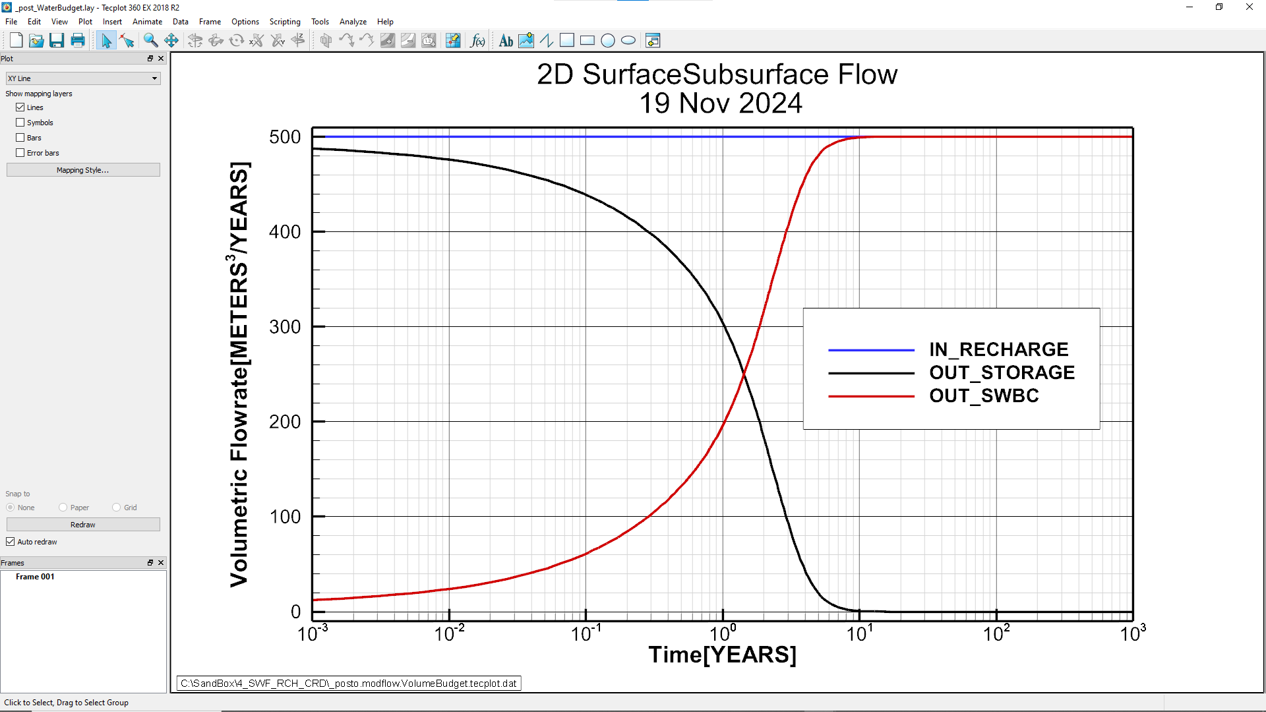
\includegraphics[width=\textwidth]{4_2_Budget}

This \tecplot\ frame has the following features and contents:
\begin{itemize}
  \item It is an {\sf XY Line} plot showing the volumetric flowrate versus time for selected components of the model.
  \item The name of the data file loaded into the frame is shown at the bottom left corner.
  \item The plot title, current date (on the day the file was loaded) and data set title ({\sf 4\_SWF\_RCH\_CRD}) are shown centred above the plot.
  \item The line legend is shown on the right side of the plot.
  \item The X-axis uses a log time scale.
\end{itemize}

The \tecplot\ date set information dialogue shows all of the variables available for plotting:

        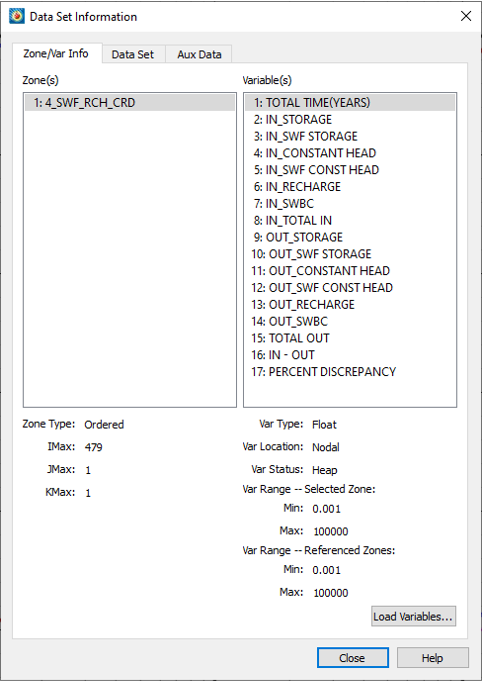
\includegraphics[width=.6\textwidth]{4_3_DataSetInfo}

Variable names are derived from the {\tt modflow.lst} file:
\begin{verbatim}
      VOLUMETRIC BUDGET FOR ENTIRE MODEL AT END OF TIME STEP  479 IN STRESS PERIOD    1
      ----------------------------------------------------------------------------- ---

         CUMULATIVE VOLUMES      L**3       RATES FOR THIS TIME STEP      L**3/T
         ------------------                 ------------------------

               IN:                                      IN:
               ---                                      ---
                 STORAGE =       3.0881E-04               STORAGE =       5.6023E-09
             SWF STORAGE =       9.9743E-03           SWF STORAGE =       2.1841E-13
           CONSTANT HEAD =           0.0000         CONSTANT HEAD =           0.0000
          SWF CONST HEAD =           0.0000        SWF CONST HEAD =           0.0000
                RECHARGE =    50000000.0000              RECHARGE =         500.0000
                    SWBC =           0.0000                  SWBC =           0.0000

                TOTAL IN =    50000000.0103              TOTAL IN =         500.0000

        ... etc

     PERCENT DISCREPANCY =           0.01     PERCENT DISCREPANCY =           0.01
\end{verbatim}


This example has a uniform recharge rate of 0.5 $meters/year$ which results in a total recharge of 500 $meters^{3}/year$ when multiplied by the 1000 $meter$ length of the cross-section. Initially, water comes out of storage then but this declines to zero at equilibrium.  Water exiting the surface water outflow critical depth boundary  {\sf OUT\_SWBC} is initially zero then rises to equal the toal recharge at equilibrium.  Fluid balance error {\sf IN-OUT} is essentially zero throughout the simulation.

The probe tool can be used in {\sf XY Line} plots to get exact variable values at a chosen location along the X or Y axis.  The cursor is shown as a vertical line if probing values on the X-axis (i.e.\ over time):

        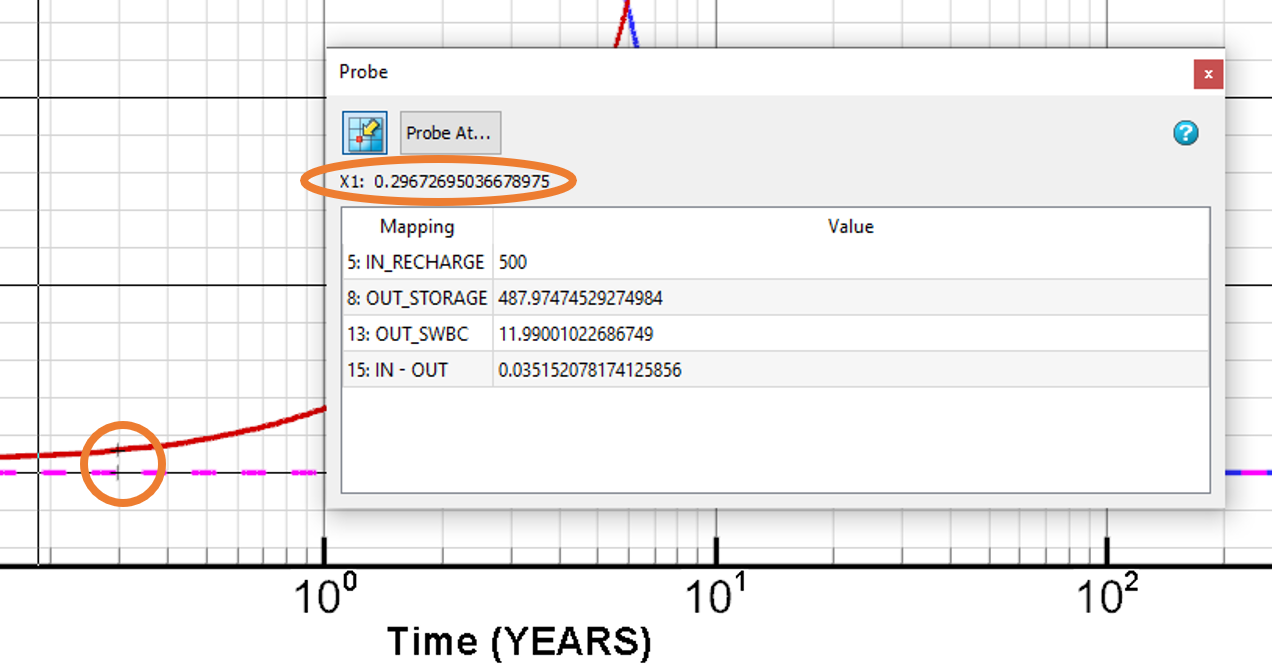
\includegraphics[width=\textwidth]{4_4_Probe}

Here, the location of the probe is shown by small vertical lines placed where the probe crossed the plotted lines.  The exact coordinate is given as {\sf X1: 0.2967...}  years.  At this early time, the {\sf OUT\_STORAGE} value is still near its initial value of 500 and the {\sf OUT\_SWBC} has just started rising.

A \tecplot\ layout file, \texttt{\_post.lay}, has been created for each verification example and  provides a quick way to view \mfus\ model solution results.  This result is from the example {\tt 6\_Abdul\_Prism\_Cell}:

        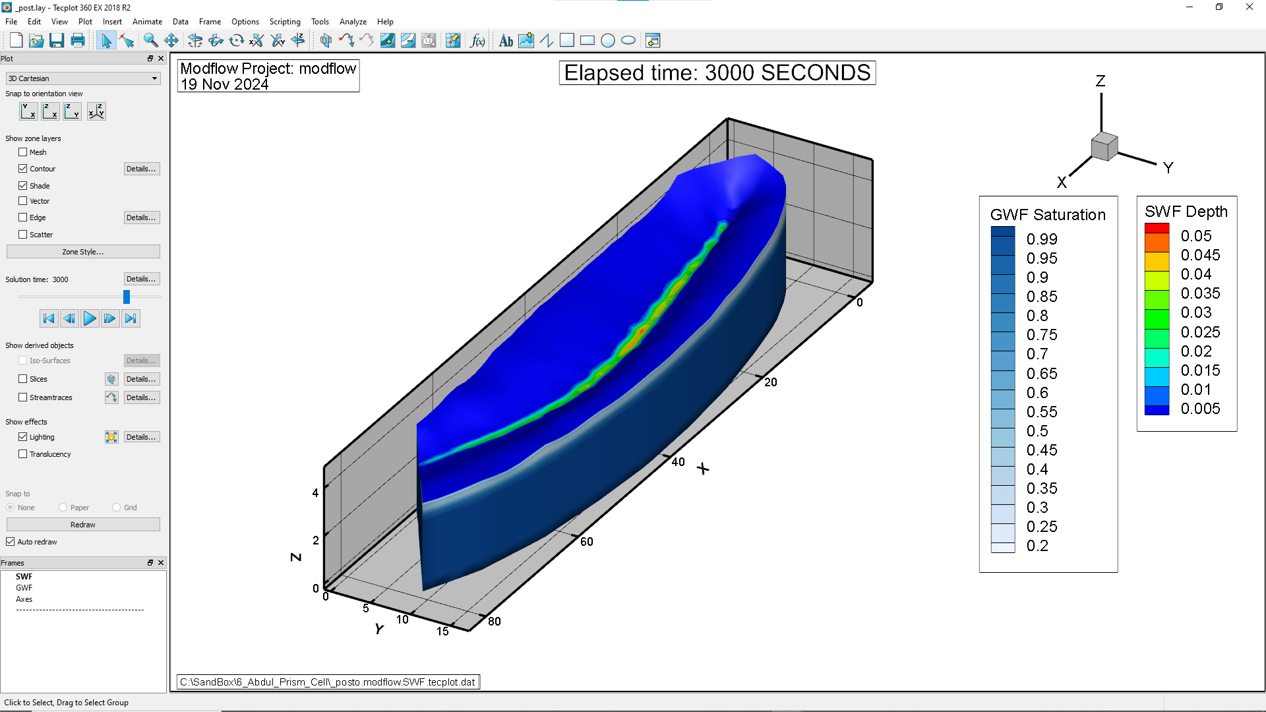
\includegraphics[width=\textwidth]{4_5_Post_Abdul}

The {\tt \_post.lay} layout file is similar to the {\tt \_build.lay} file shown earlier for the same problem: {\sf  SWF, GWF} and {\sf Axes} frames are visible (i.e. placed above the {\sf background} frame in the list).  The {\sf SWF} is currently active (i.e. the name is bolded) and placed at the front of the image (i.e. at the top of the list). It uses a different colormap to make it easier to distinguish the \gwf\ domain below.

In this case though, the contoured variables are {\sf SWF Depth} and {\sf GWF Saturation} results from the \mfus\ simulation.  The model output includes data for several output times, and the image above is showing conditions at a solution time of 3000 seconds, as indicated by the label near the top center of the plot.  The solution time shown is controlled by the slider and button controls near the centre of the {\sf Plot} frame on the left hand side of the image:

        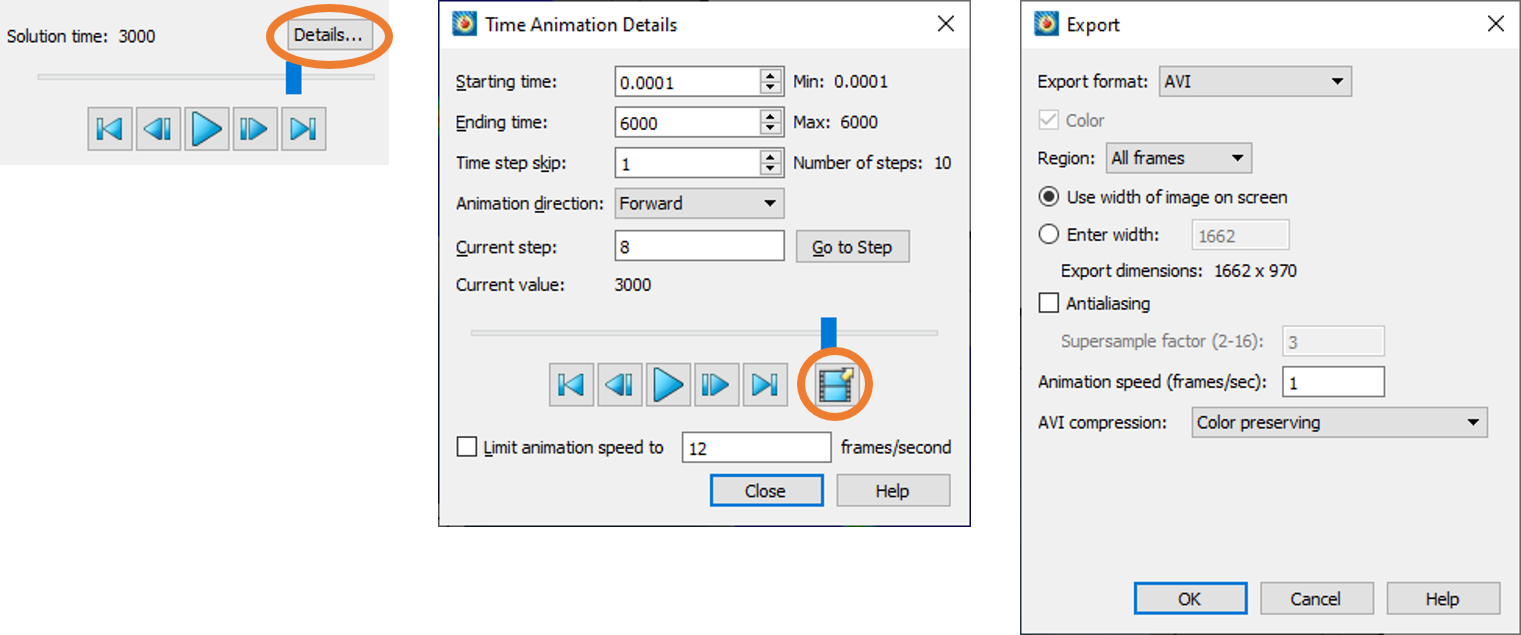
\includegraphics[width=.8\textwidth]{4_6_SolutionSlider}

The {\sf Details...} button leads to the {\sf Time animation details} dialogue which allows you to control and save animations of transient model results using the {\sf Export To File} button 
\includegraphics{ExportToFile}.  There is an example animation in  \texttt{$\backslash$MUT\_Examples-main$\backslash$\-6\_Abdul\_Prism\_Cell} folder in the powerpoint file {\tt Abdul Problem Animation.pptx}.  It used the settings shown in the {\sf Export} dialogue above to limit animations speed and write to an {\tt AVI}-formatted file.  This was then inserted in powerpoint where it can be viewed.

The {\sf Data Set Information} dialogues for the {\sf SWF} and {\sf GWF} frames are shown below:

        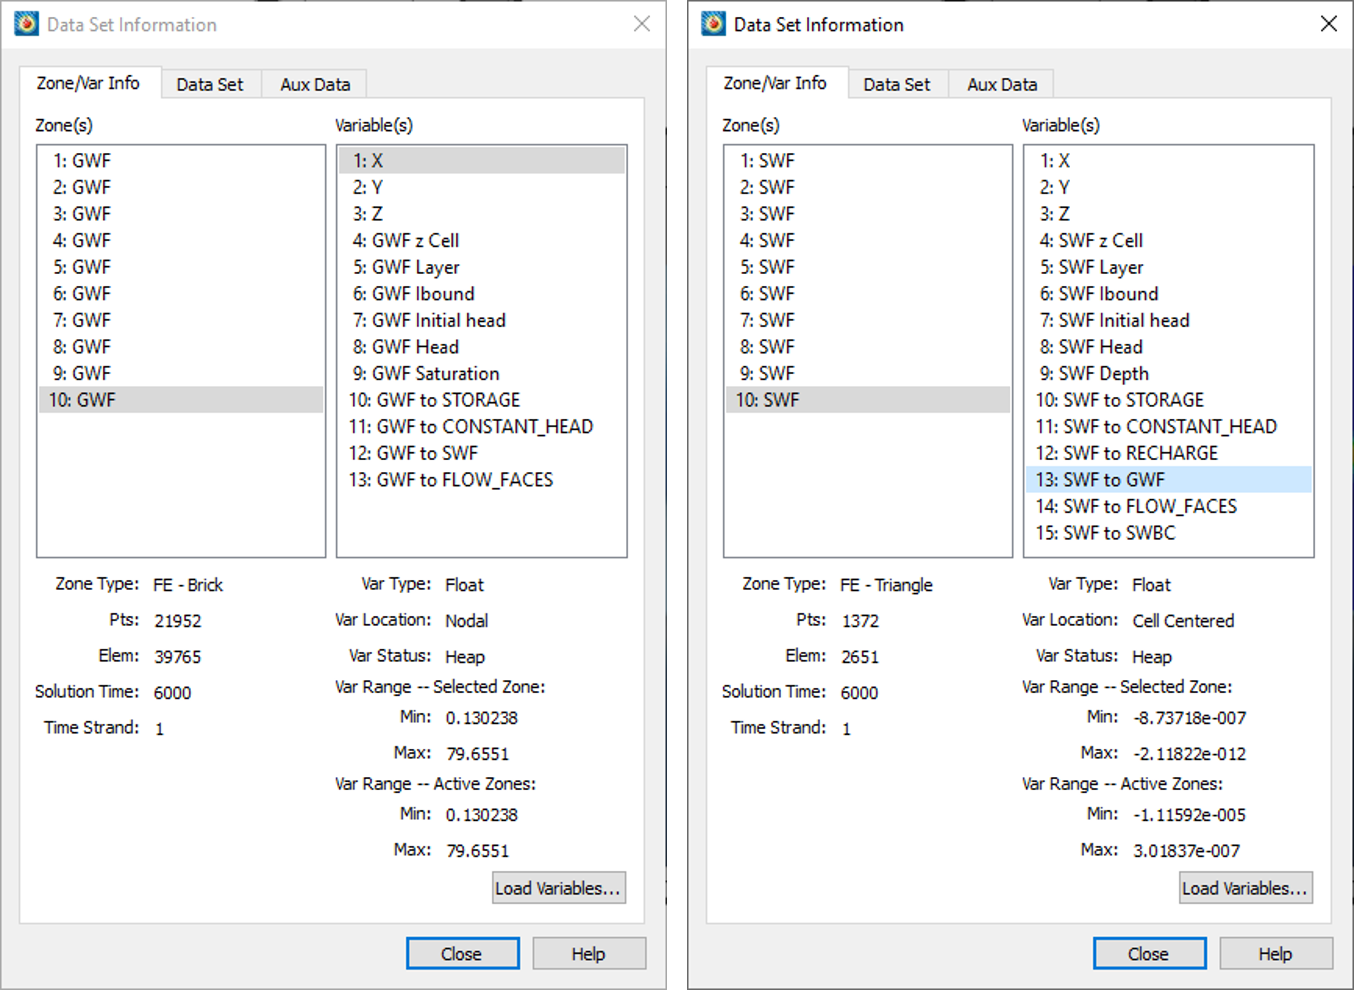
\includegraphics[width=.8\textwidth]{4_7_DatSetInfo}

These are similar to those shown earlier during the model build except there are now multiple {\sf Zone(s)}, one for each output time.  The {\sf Solution Time} (6000) is shown for the highlighted zone, in this case zone 10.

Included are these cell properties:
\begin{itemize}
    \item Elevation {\sf SWF z Cell} and {\sf GWF z Cell}.
    \item \mf\ layer number  {\sf SWF layer}and {\sf GWF layer}.
    \item \mf\ boundary number {\sf SWF Ibound} and {\sf GWF Ibound}.
    \item Initial head.
    \item Hydraulic head result.
    \item \gwf\ saturation and \swf\ depth.  These are stored in the \mf\ DDN (drawdown) file.
    \item In this case, cell-by-cell flows are stored in \gwf\ variables 10 to 13 and \swf\ variables 10 to 15.
\end{itemize}

The verification example {\tt 6\_Abdul\_MODHMS} layout file {\sf \_plot.lay} uses \tecplot\ value-blanking and the {\sf SWF Ibound} and {\sf GWF Ibound} to remove inactive cells, which have an IBOUND value of 0, from the plot:

        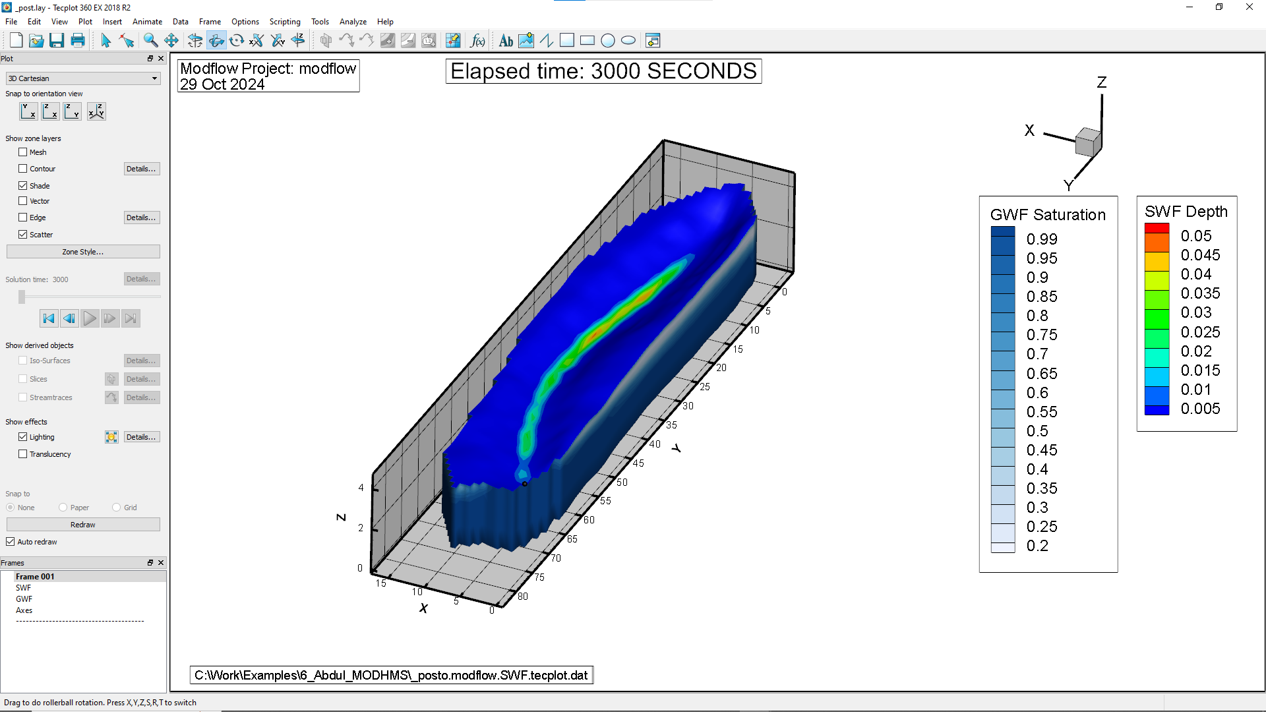
\includegraphics[width=.8\textwidth]{4_7a_MODHMS}


        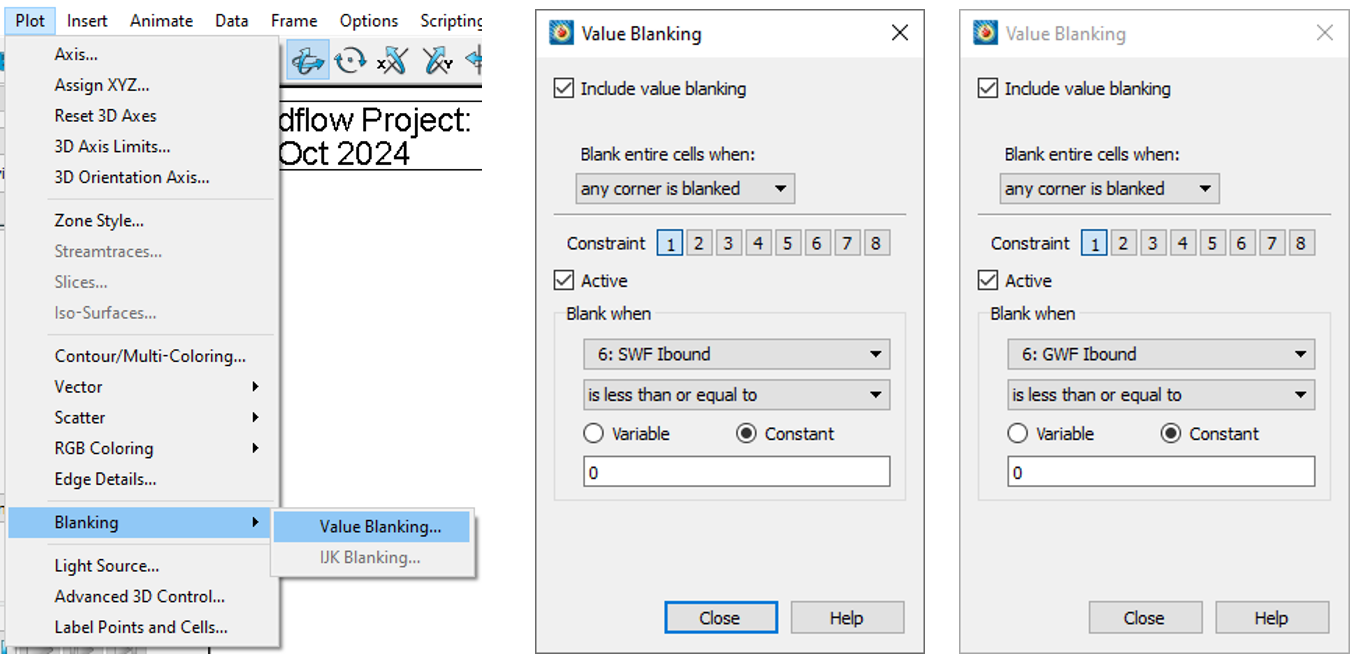
\includegraphics[width=.8\textwidth]{4_7b_ValueBlanking}

\index{\tecplot\ ! value blanking} 


        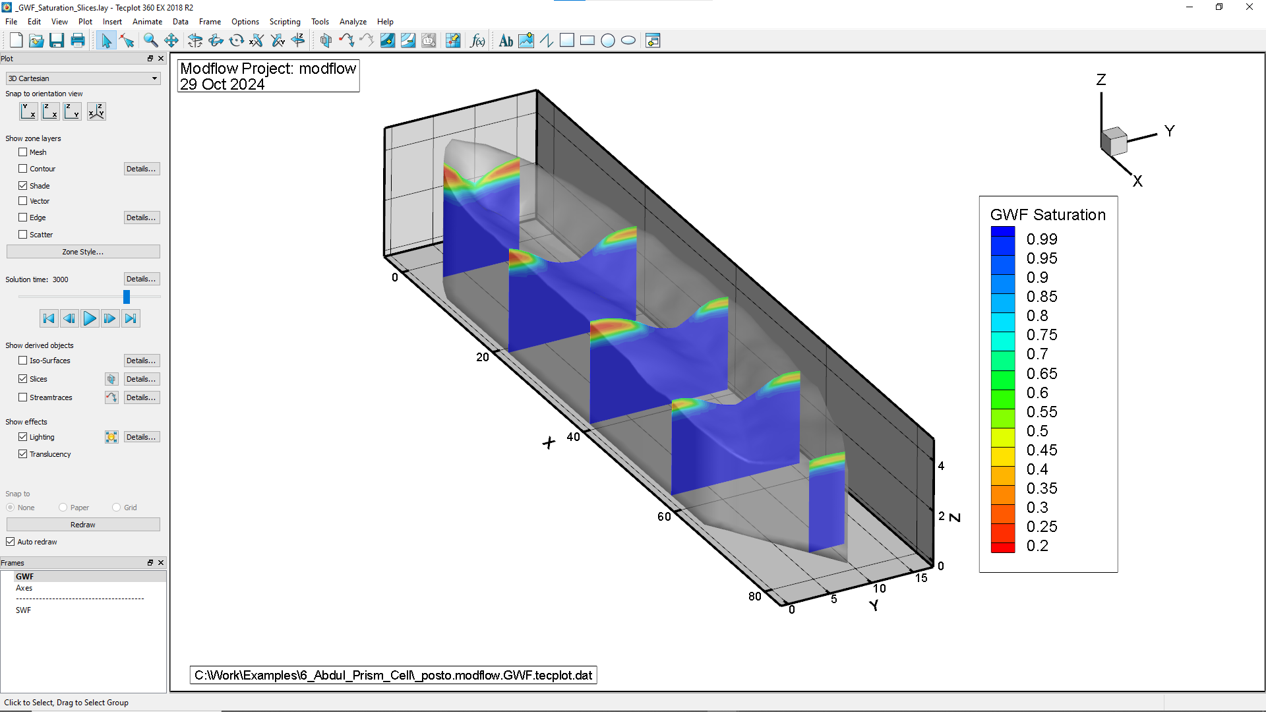
\includegraphics[width=.8\textwidth]{4_8_Slices}

\index{\tecplot\ ! slices and Fence diagrams}

